\documentclass[tikz]{standalone}

\usetikzlibrary{shapes,arrows}

\tikzstyle{block} = [rectangle, draw, fill=blue!20, text width=5em, text centered, rounded corners, minimum height=4em]
\tikzstyle{line} = [draw, -latex']

\begin{document}

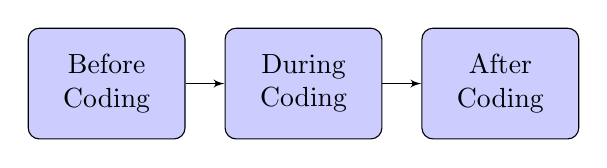
\begin{tikzpicture}[node distance = 2.5cm, auto]
    % Place nodes
    \node [block] (before) {Before Coding};
    \node [block, right of=before] (during) {During Coding};
    \node [block, right of=during] (after) {After Coding};
    % Draw edges
    \path [line] (before) -- (during);
    \path [line] (during) -- (after);
\end{tikzpicture}

\end{document}